%========================================================
% Appendix (thesis): Noise and Errors — Extended Analysis and Full Results
%========================================================
\section{Qiskit Simulation}
\label{appendix:qiskit-simulation}

\begin{figure}[ht!]
    \centering
    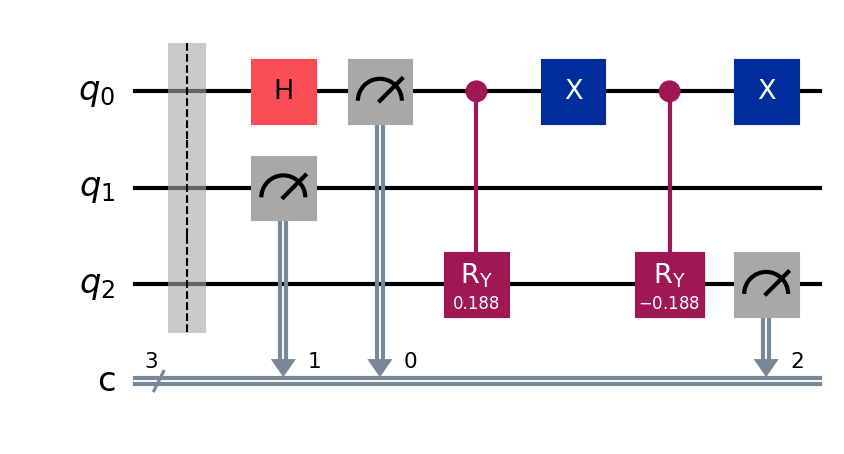
\includegraphics[width=0.45\textwidth]{Appendix/plots/qcs/H1_B_qc.png}
    \caption{Quantum circuit measuring the local term \( H_b \) in the energy teleportation protocol.}
    \label{fig:H1_qc}
\end{figure}

\begin{figure}[ht!]
    \centering
    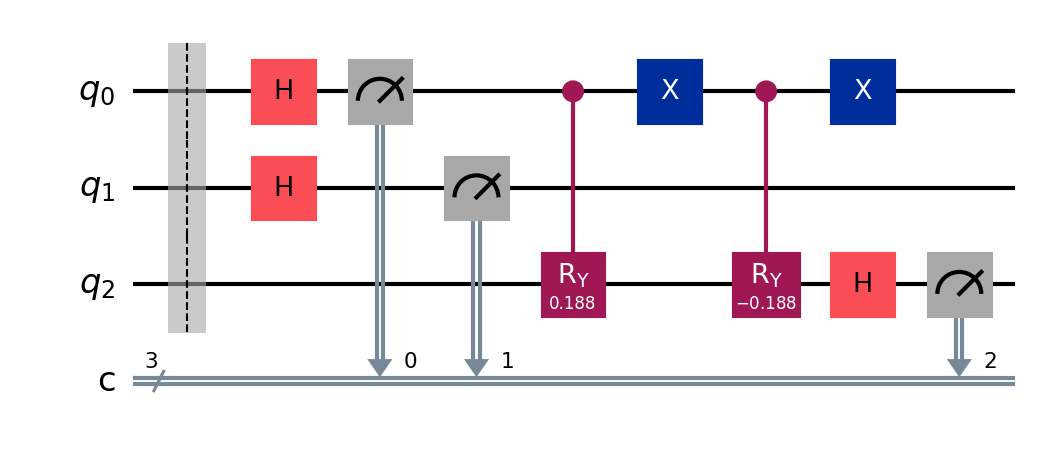
\includegraphics[width=0.45\textwidth]{Appendix/plots/qcs/V_B_qc.png}
    \caption{Quantum circuit measuring the interaction term \( V_{ab} \) in the energy teleportation protocol.}
    \label{fig:V_qc}
\end{figure}

This appendix presents the quantum circuits used throughout this work. We include the energy-teleportation components \(H_1\) and \(V\), each measured at Bob’s site. As discussed in Section~\ref{sec:complex-sum-constructed-operator}, \([H_1,V]\neq 0\), so \(H_1\) and \(V\) must be evaluated in two separate circuits. The circuit designs closely follow Ikeda’s implementation of quantum energy teleportation on superconducting hardware~\cite{Ikeda2023}.
